\documentclass[a4paper,12pt]{article} % добавить leqno в [] для нумерации слева
\usepackage[a4paper,top=1.3cm,bottom=2cm,left=1.5cm,right=1.5cm,marginparwidth=0.75cm]{geometry}
%%% Работа с русским языком
\usepackage{cmap}					% поиск в PDF
\usepackage{mathtext} 				% русские буквы в фомулах
\usepackage[T2A]{fontenc}			% кодировка
\usepackage[utf8]{inputenc}			% кодировка исходного текста
\usepackage[english,russian]{babel}	% локализация и переносы

\usepackage{graphicx}

\usepackage{wrapfig}
\usepackage{tabularx}

\usepackage{hyperref}
\usepackage[rgb]{xcolor}
\hypersetup{
colorlinks=true,urlcolor=blue
}
\usepackage{multirow}
\usepackage{hhline}


%%% Дополнительная работа с математикой
\usepackage{amsmath,amsfonts,amssymb,amsthm,mathtools} % AMS
\usepackage{icomma} % "Умная" запятая: $0,2$ --- число, $0, 2$ --- перечисление

%% Номера формул
\mathtoolsset{showonlyrefs=true} % Показывать номера только у тех формул, на которые есть \eqref{} в тексте.

%% Шрифты
\usepackage{euscript}	 % Шрифт Евклид
\usepackage{mathrsfs} % Красивый матшрифт

%% Свои команды
\DeclareMathOperator{\sgn}{\mathop{sgn}}

%% Перенос знаков в формулах (по Львовскому)
\newcommand*{\hm}[1]{#1\nobreak\discretionary{}
{\hbox{$\mathsurround=0pt #1$}}{}}

\begin{document}
	
	\begin{titlepage}
	\begin{center}
		{\large МОСКОВСКИЙ ФИЗИКО-ТЕХНИЧЕСКИЙ ИНСТИТУТ (НАЦИОНАЛЬНЫЙ ИССЛЕДОВАТЕЛЬСКИЙ УНИВЕРСИТЕТ)}
	\end{center}
	\begin{center}
		{\large Физтех-школа электроники, фотоники и молекулярной физики}
	\end{center}
	
	
	\vspace{4.5cm}
	{\huge
		\begin{center}
			{Лабораторная работа 4.3.3}\\
			Исследование разрешающей способности микроскопа методом Аббе
		\end{center}
	}
	\vspace{2cm}
	\begin{flushright}
		{\LARGE Салтыкова Дарья \\
			\vspace{0.5cm}
			Б04-105}
	\end{flushright}
	\vspace{8cm}
	\begin{center}
		Долгопрудный 2023
	\end{center}
\end{titlepage}

\section{Введение}

\noindent \textbf{Цель работы:} Определение дифракционного предела разрешения
объектива микроскопа методом Аббе.

\medskip

\noindent \textbf{В работе используются:} лазер, кассета с набором сеток разного
периода, линзы, щель с микрометрическим винтом, оптический стол
c набором рейтеров и крепёжных винтов, экран, линейка.


\section{Теоретические сведения}
\noindent Разрешающей способностью оптического прибора называют минимальное расстояние $l_{min}$ между двумя точками в пространстве предметов, которое прибор может разрешить. При визуальном наблюдении изображения в качестве критерия разрешения применяют так называемый критерий Рэлея. 

\medskip

\noindent Для иммерсионного микроскопа (объект находится в иммерсионной среде — жидкости с показателем преломления n) разрешающая способность объектива при некогерентном освещении
\begin{equation}
    l_{min} = \frac{0.61 \lambda}{n \sin A},
\end{equation}

\noindent где A — апертурный угол объектива микроскопа. 

\medskip

\noindent Рассмотрим теперь когерентно освещённый объект, наблюдаемый в микроскоп. Схема образования изображения в объективе микроскопа
представлена на рис. 1.
    \begin{figure}[h]
    \centering
    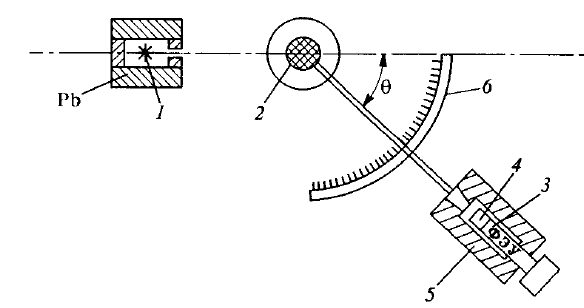
\includegraphics[width=15cm]{fig2.PNG}
    \caption{Образование изображения в объективе микроскопа. $P_1$ — плоскость предмета, $F$ — задняя фокальная плоскость объектива, $P_2$ — плоскость,
сопряжённая с предметной плоскостью. В плоскости $P_2$ световые пучки
сильно перекрываются}
    \label{fig:vac}
\end{figure}

\noindent Минимальное разрешаемое объективом расстояние
определяется условием

\begin{equation}
    l_{min} = \frac{\lambda}{\sin A} \approx \frac{\lambda}{D/2f},
\end{equation}

\noindent где D — диаметр диафрагмы. При этом диафрагма, расположенная
симметрично, пропускает нулевой и ±1 дифракционные максимумы.


\section{Экспериментальная установка}

\noindent Схема модели проекционного микроскопа приведена на рис. 2. Предметом служат сетки, расположенные
в кассете. Смена сеток осуществляется поворотом внешнего кольца кассеты.

    \begin{figure}[h]
    \centering
    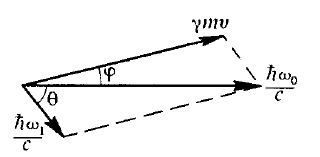
\includegraphics[width=15cm]{fig1.PNG}
    \caption{Схема экспериментальной установки — модель проекционного
микроскопа}
    \label{fig:vac}
\end{figure}


\section{Ход работы}

 \subsection{Определение периода решёток по их пространственному спектру}
 
\begin{figure}[h]
    \centering
    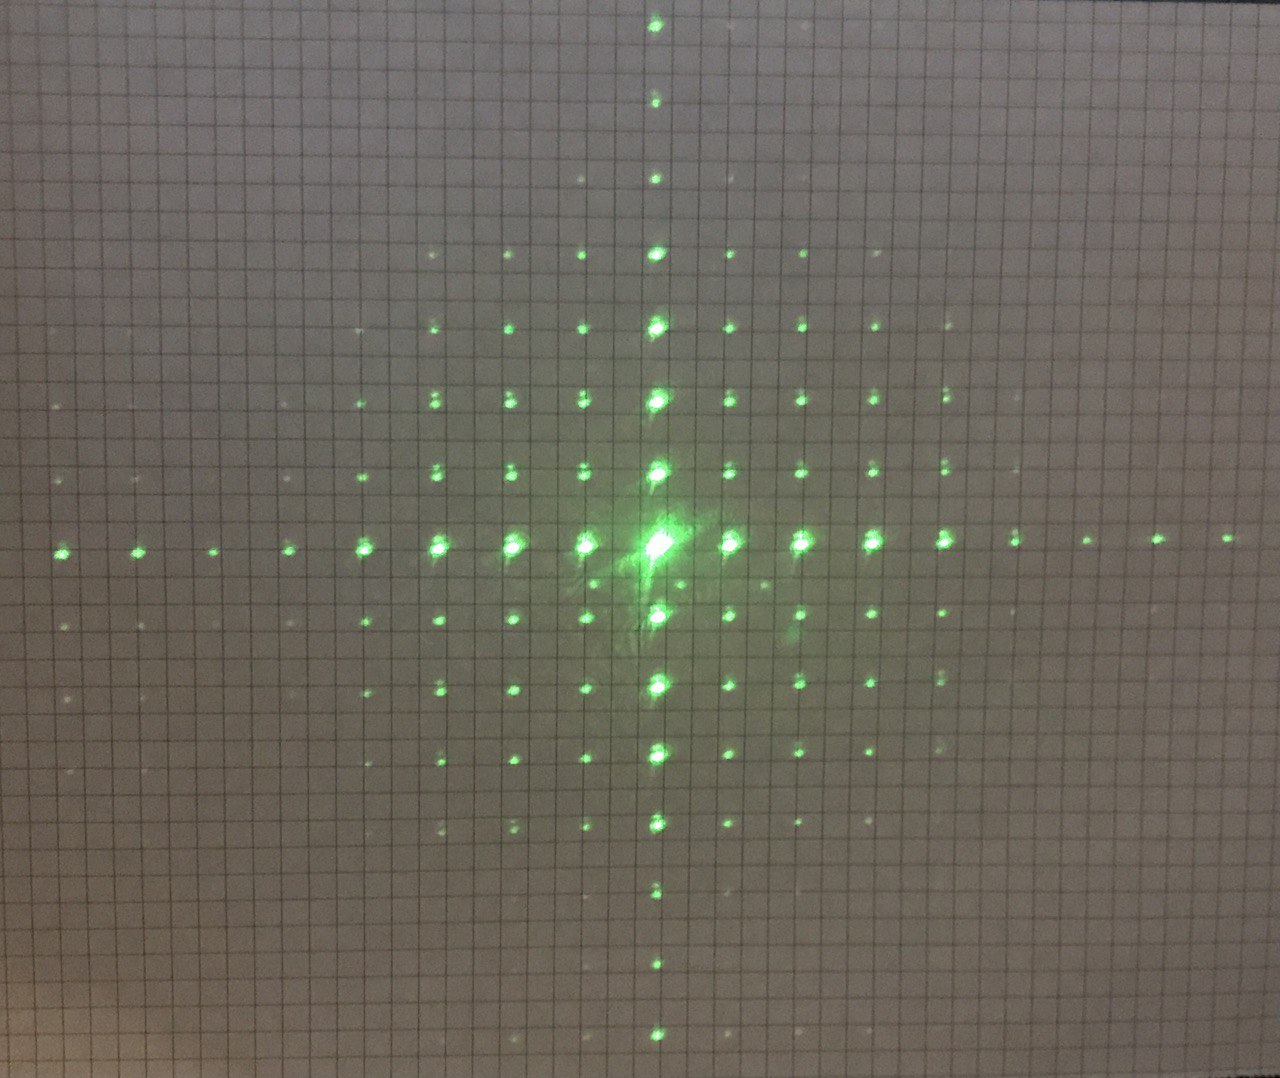
\includegraphics[width=8cm]{1.jpg}
    \label{filtr}
\end{figure}

\noindent Для определения периода решётки измерим расстояния между максимумами разных порядков на экране. Расстояние от сетки до экрана $H = 124.4$ см. Период решётки рассчитывается по формуле 
    \begin{equation}
        d = \frac{\lambda H}{d_{m}},
    \end{equation}
    
\noindent где $\lambda = 532 \text{ нм}.$

\medskip

\noindent Получим: $d = (55,2 \pm 1,2) \text{ мкм}.$

\subsection{Определение периода решеток по изображению, увеличенному с помощью модели микроскопа}


    


\noindent Соберём модель проекционного микроскопа, центрируем систему. Увеличение полученной системы вычисляется по формуле
    \begin{equation}
        \gamma = \frac{b_1 b_2}{a_1 a_2}.
\end{equation}

\newpage

\begin{table}[h!]
\begin{tabular}{|l|l|}
\hline
$a_1, \text{ мм}$  & 168      \\ \hline
$b_1, \text{ мм}$  & 355      \\ \hline
$a_2, \text{ мм}$  & 25       \\ \hline
$b_2, \text{ мм}$  & 692      \\ \hline
$\gamma$          & 58,5    \\ \hline
$d_m, \text{ мм}$ & 3,21     \\ \hline
$d, \text{ мкм}$  & 54,95 \\ \hline
\end{tabular}
\end{table}

\begin{figure}[h]
    \centering
    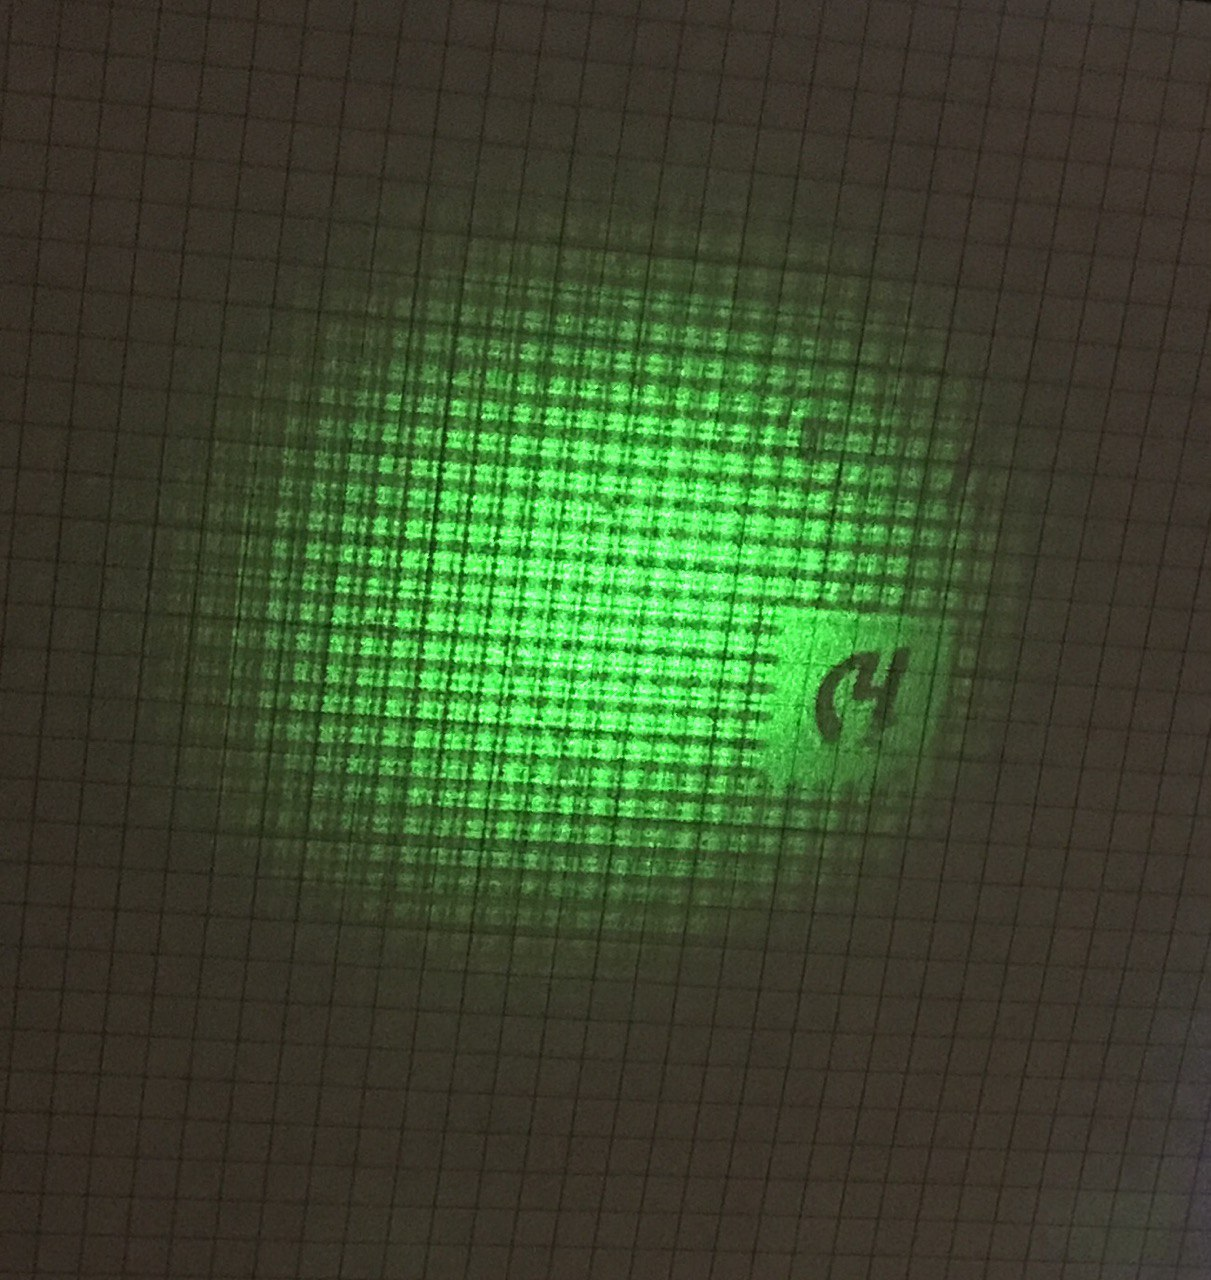
\includegraphics[width=8cm]{2.jpg}
        \label{filtr}
\end{figure}

\subsection{Пространственная фильтрация и мультиплицирование}

\noindent Поворачивая щель относительно оси, добьёмся того, чтобы щель занимала наклонное положение под $45^\circ$. Тогда будет осуществляться пространственная фильтрация, то есть выделение из спектра максимумов $m_x = m_y$ (диагональных максимумов). Тогда на экране возникнет изображение решётки, которой нет на самом деле. Полосы располагаются под углом $45^\circ$, что видно на рисунке. Период новой решетки равен в $\sqrt{2}$ раз больше периода изображения решётки, определённого стандартным методом (по увеличенному изображению решётки). Это объясняется тем фактом, что расстояние между выделенными максимумами, то есть между вторичными источниками волн, составляет $d\sqrt{2}$. Также наблюдали мультиплицирование, то есть рассечение фурье-образа щели сеткой. Такой эффект создаётся, если в нашей установке поменять местами сетку и щель.

\begin{figure}[h]
    \centering
    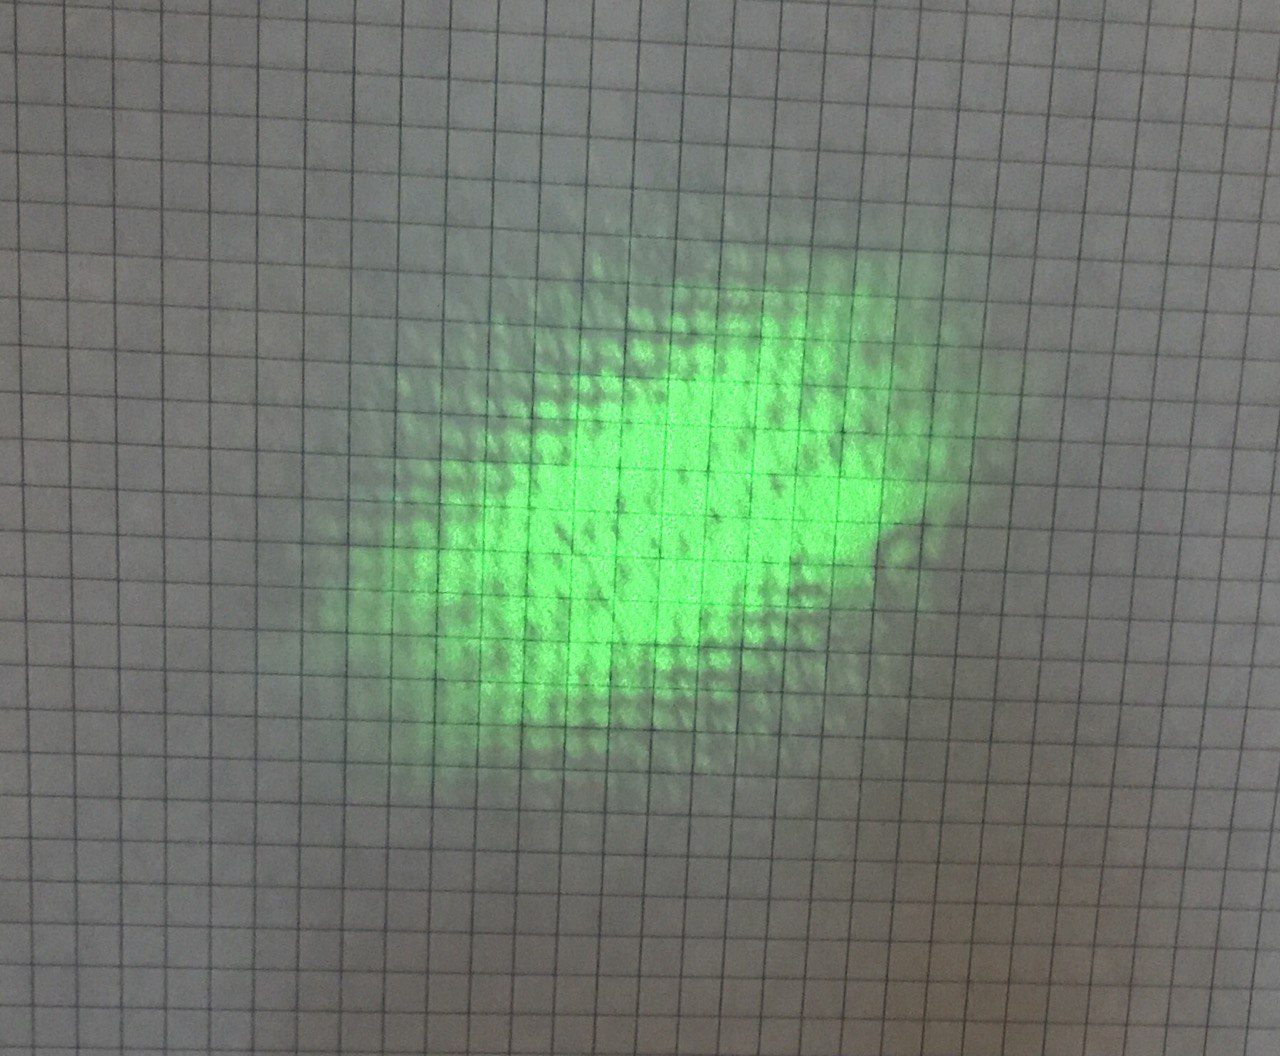
\includegraphics[width=8cm]{3.jpg}
    \caption{Пространственная фильтрация}
    \label{filtr}
\end{figure}



\newpage


\section{Вывод}

\noindent В ходе работы был измерен период дифракционной решётки двумя  способами: по пространственному спектру $(55,2 \pm 1,2) \text{ мкм}$ и изображению с микроскопа $(54,9 \pm 1,4) \text{ мкм}$. Результаты измерений практически совпадают. 




\end{document}